\documentclass[12pt]{article}
\usepackage{fullpage,graphicx,psfrag,amsmath,amsfonts,verbatim}
\usepackage[small,bf]{caption}

\input defs.tex

\bibliographystyle{alpha}

\title{Assignment 3 CME 241}
\author{Taylor Howell}

\begin{document}
\maketitle

\paragraph{1.} Bellman Policy Equations (discrete policy).
$$V^{\pi_D} = \mathcal{R}^{\pi_D}(s) + \gamma \sum\limits_{s' \in \mathcal{N}} \mathcal{P}^{\pi_D}(s, s') \cdot V^{\pi_D}(s')$$

$$Q^{\pi_D}(s,a) = \mathcal{R}^{\pi_D}(s, a) + \gamma \sum\limits_{s' \in \mathcal{N}} \mathcal{P}^{\pi_D}(s, s') \cdot Q^{\pi_D}(s', a')$$

$$Q^{\pi_D}(s,a) = \mathcal{R}^{\pi_D}(s, a) + \gamma \sum\limits_{s' \in \mathcal{N}} \mathcal{P}^{\pi_D}(s, s') \cdot V^{\pi_D}(s')$$

$$V^{\pi_D}(s) = \mathcal{R}^{\pi_D}(s) + \gamma \sum\limits_{s' \in \mathcal{N}} \mathcal{P}^{\pi_D}(s, s') \cdot Q^{\pi_D}(s',\pi_D(s'))$$

\paragraph{2.}
The Bellman Optimality Equation:
$$ V^{*}(s) = \underset{a \in \mathcal{A}}{\mbox{max}} \{\mathcal{R}(s,a) + \gamma \sum\limits_{s' \in \mathcal{N}} \mathcal{P}(s,a,s') \cdot V^{*}(s')\}$$
\begin{align*}
	\mathcal{R}(s,a) &= \sum\limits_{s' \in \mathcal{N}} \mathcal{P}(s,a,s') \cdot \mathcal{R}(s,a,s') \\
	&= a (1 - a) + (1 - a) (1 + a)\\
	&= a - a^2 + 1 - a^2 \\
	&= -2 a^2 + a + 1
\end{align*}

\begin{align*}
	 \gamma \sum\limits_{s' \in \mathcal{N}} \mathcal{P}(s,a,s') \cdot V^{*}(s') &= \gamma a V^{*}(s') + \gamma (1 - a) V^{*}(s)\\
	 &= \gamma a y  + \gamma x - \gamma a x, \quad \mbox{where: } x = V^{*}(s), y = V^{*}(s+1)
\end{align*}

$$ f(a) = -2 a^2 + (1 + \gamma y - \gamma x) a + (1 + \gamma x)$$

Set $\frac{\partial f}{\partial a} = 0$, solving $\rightarrow a^{*} = \frac{1 + \gamma (y - x)}{4}$. The optimal deterministic policy:
$$\pi_D = \frac{1 + \gamma \Big(V^{*}(s+1) - V^{*}(s)\Big)}{4}$$

Plugging into this result back into the Optimality Equation, $f(a) = 1 + \gamma x - \frac{-(1 + \gamma (y - x)^2)}{16}$:

$$V^{*}(s) = 1 + \gamma V^{*}(s) - \frac{(1 + \gamma (V^{*}(s+1) - V^{*}(s))^2)}{16}$$.

(needs a relationship between $V(s)$ and $V(s+1)$).

\paragraph{3.} Frog escape. For a scenario with $n$ lilypads, the state space and terminal states are: 
$$\mathcal{S} : \{0, \dots, n\}, \quad \mathcal{T} : \{0, n\},$$
and the action space is:
$$\mathcal{A} : \{A, B\}.$$ For non-terminal states, i.e., $S_t \in \mathcal{S} - \mathcal{T}$, the transition probabilities are:
$$\mathcal{P}(S_{t+1} = i-1 | S_t = i, A_t = A) = \frac{i}{n}$$
$$\mathcal{P}(S_{t+1} = i+1 | S_t = i, A_t = A) = \frac{n-i}{n}$$
$$\mathcal{P}(S_{t+1} = j,\,\mbox{for}\, j \in \{0, \dots, n\} | S_t = i, A_t = B) = \frac{1}{n}$$
The reward function is:
$$\mathcal{R}(S_t = 0, a) = 0 $$
$$\mathcal{R}(S_t = n, a) = +1 $$
$$\mathcal{R}(S_{t} = j,\,\mbox{for}\,j \in \{1, \dots, n-1\}, a) = 0 $$
See $\texttt{frog\_escape.py}$.

\begin{figure}[h]
	\centering
	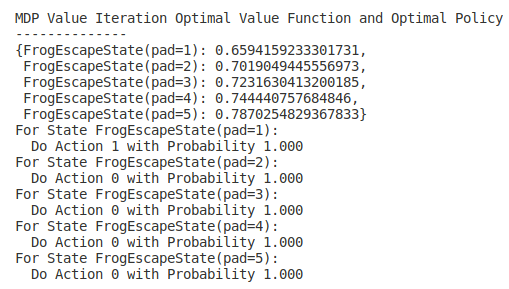
\includegraphics[width=.5\textwidth]{frog_escape_n6.png}
	\caption{The optimal policy and value function--corresponding to the probability of escape--for Frog escape problem with $n = 6$.}
\end{figure}
(See the printouts from my code for optimal policies.)

The optimal policy selects action $A$ for all states $s_t != 1$. In this case it is too risky to possibly select an action that may decrement (to the snake!) with probability $(\frac{i}{n}$. The probability of not ending up with the snake is the same for $A$ and $B$ in this state, but it's optimal to select $B$ since this may be closer to state $n$.

By setting the reward to $r_t = 1$ for escaping, along with discount factor $\gamma = 1$, the value function at each state is the probability of escape. 

\paragraph{4.} 

I utilized the following Stack Exchange post to compute the expected value https://math.stackexchange.com/questions/176196/calculate-the-expected-value-of-y-ex-where-x-sim-n-mu-sigma2. Once the expected value is computed, the log of the expectation can be minimized (since log is monotonic) and the optimal action $a^*$ can be plugged back into the expected value to compute the corresponding optimal cost.


\begin{figure}
	\centering
	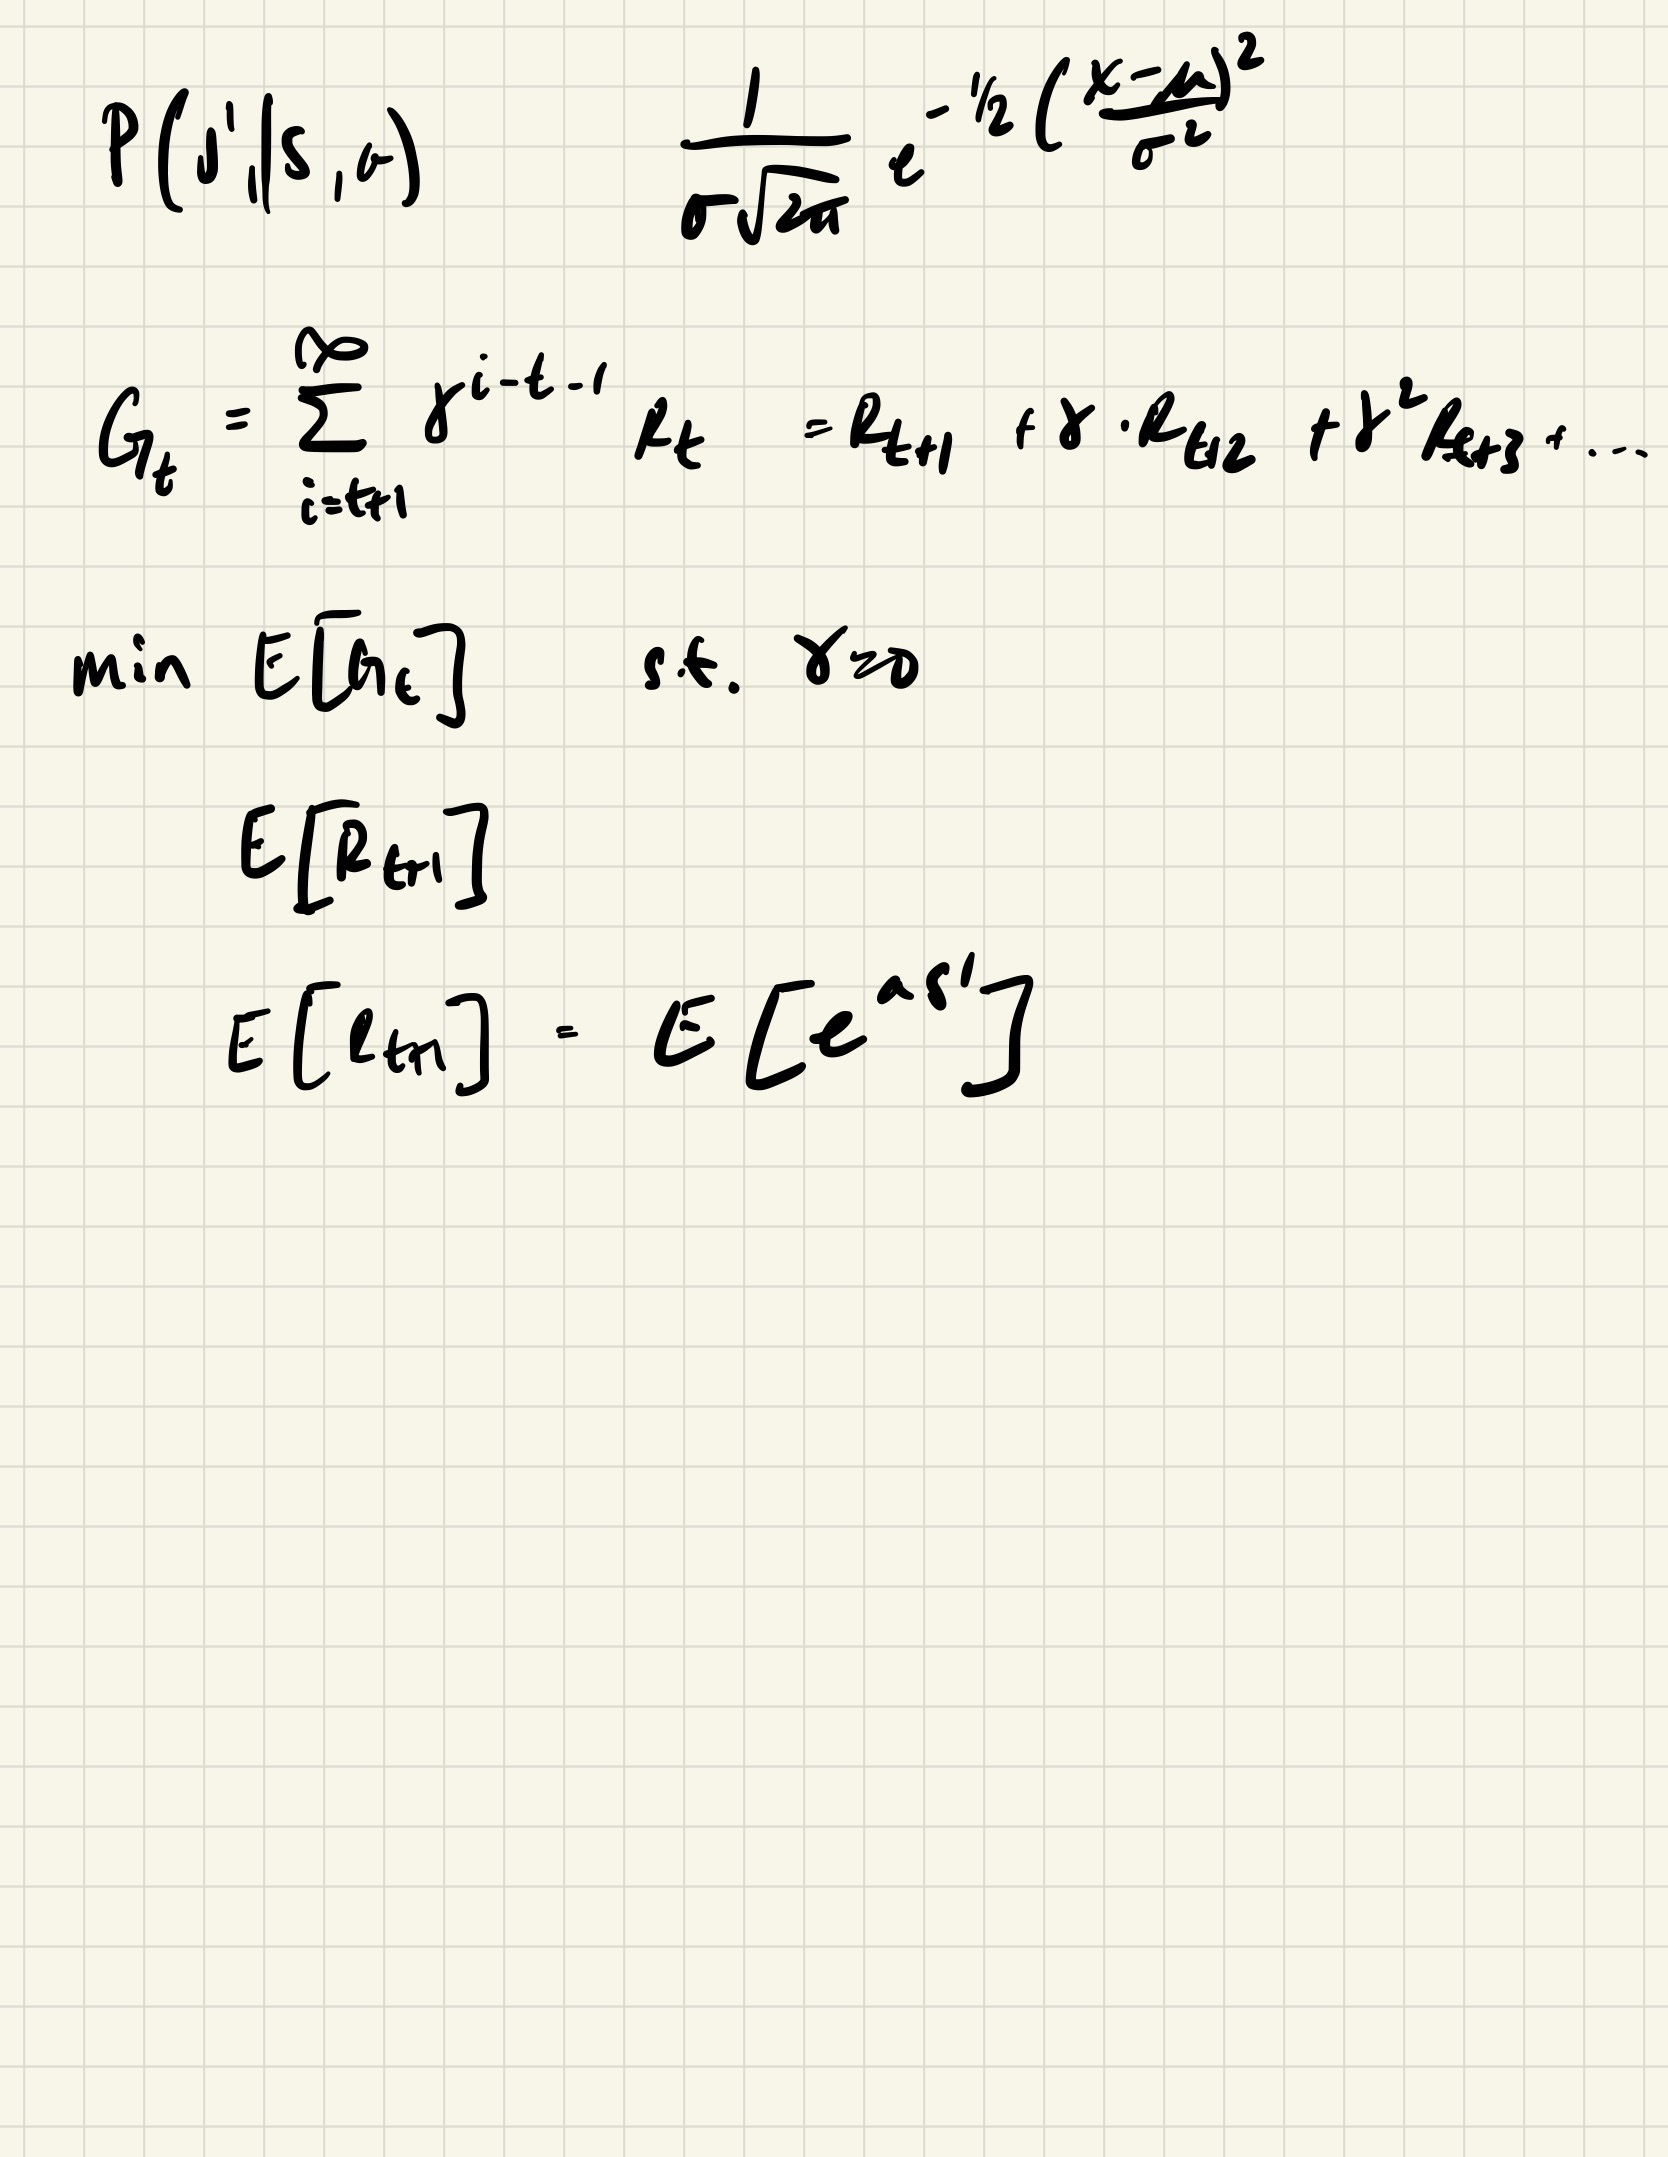
\includegraphics[width=.5\textwidth]{q4_1.jpg}
\end{figure}
\begin{figure}
	\centering
	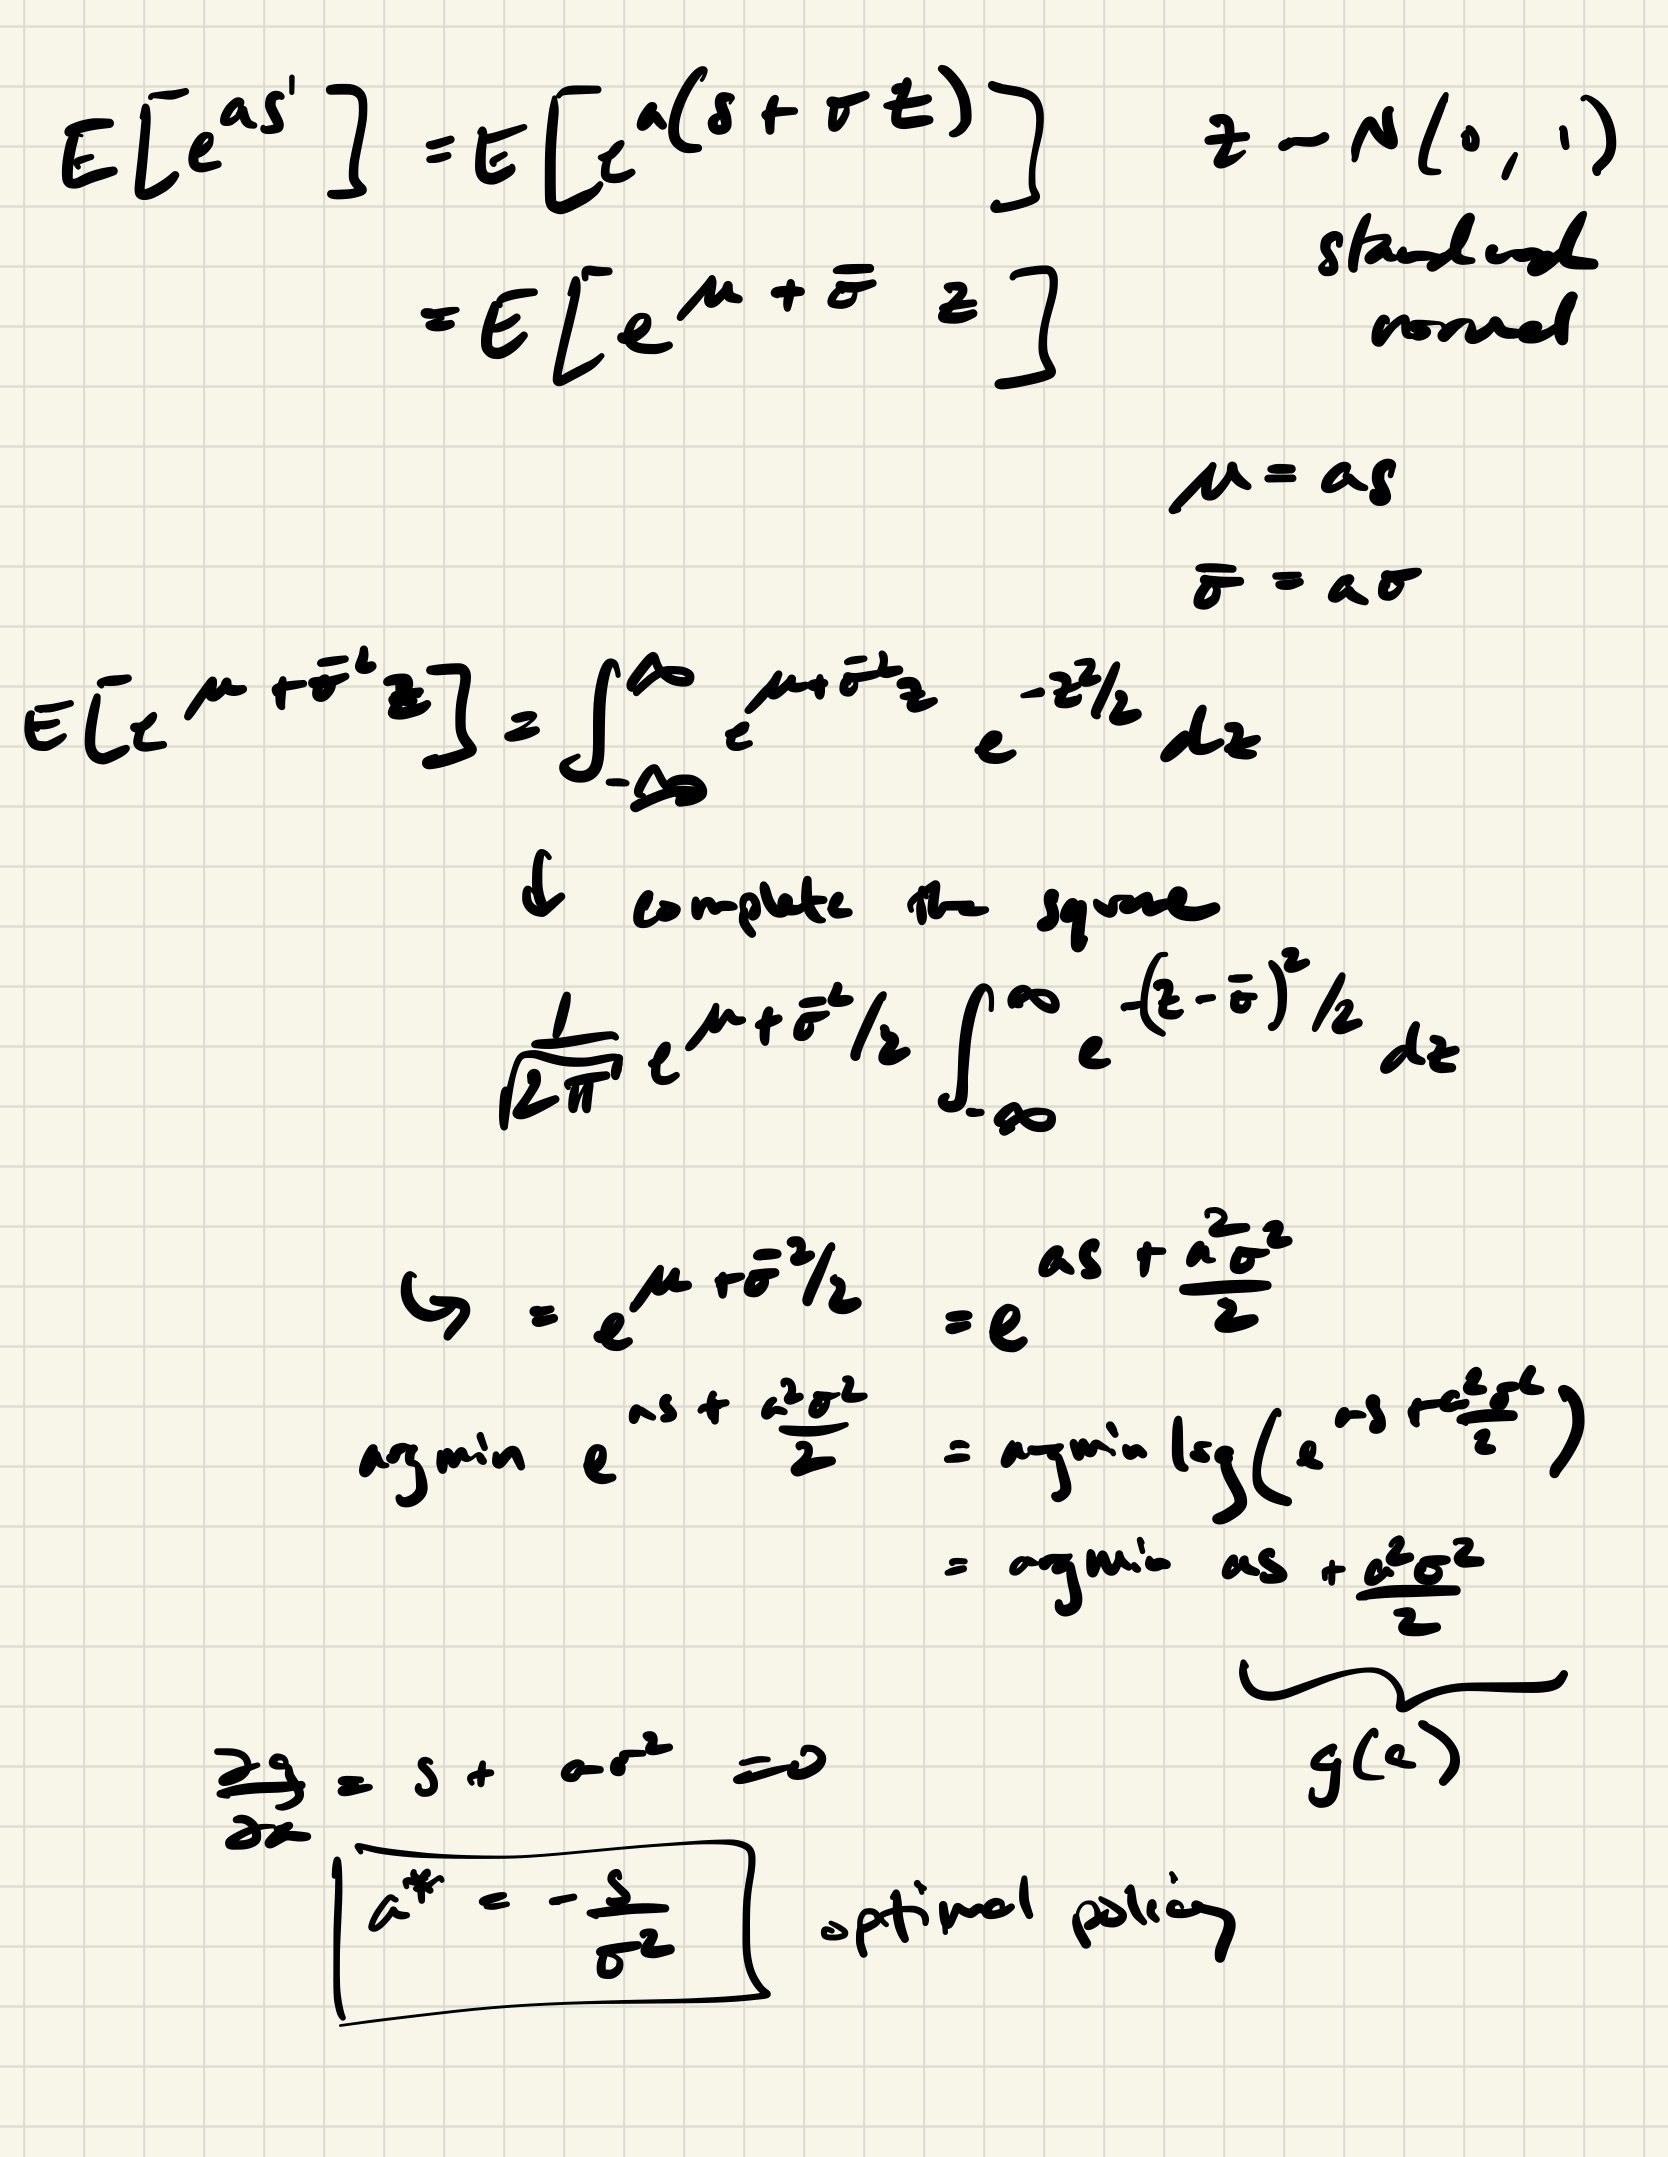
\includegraphics[width=.5\textwidth]{q4_2.jpg}
\end{figure}
\begin{figure}
	\centering
	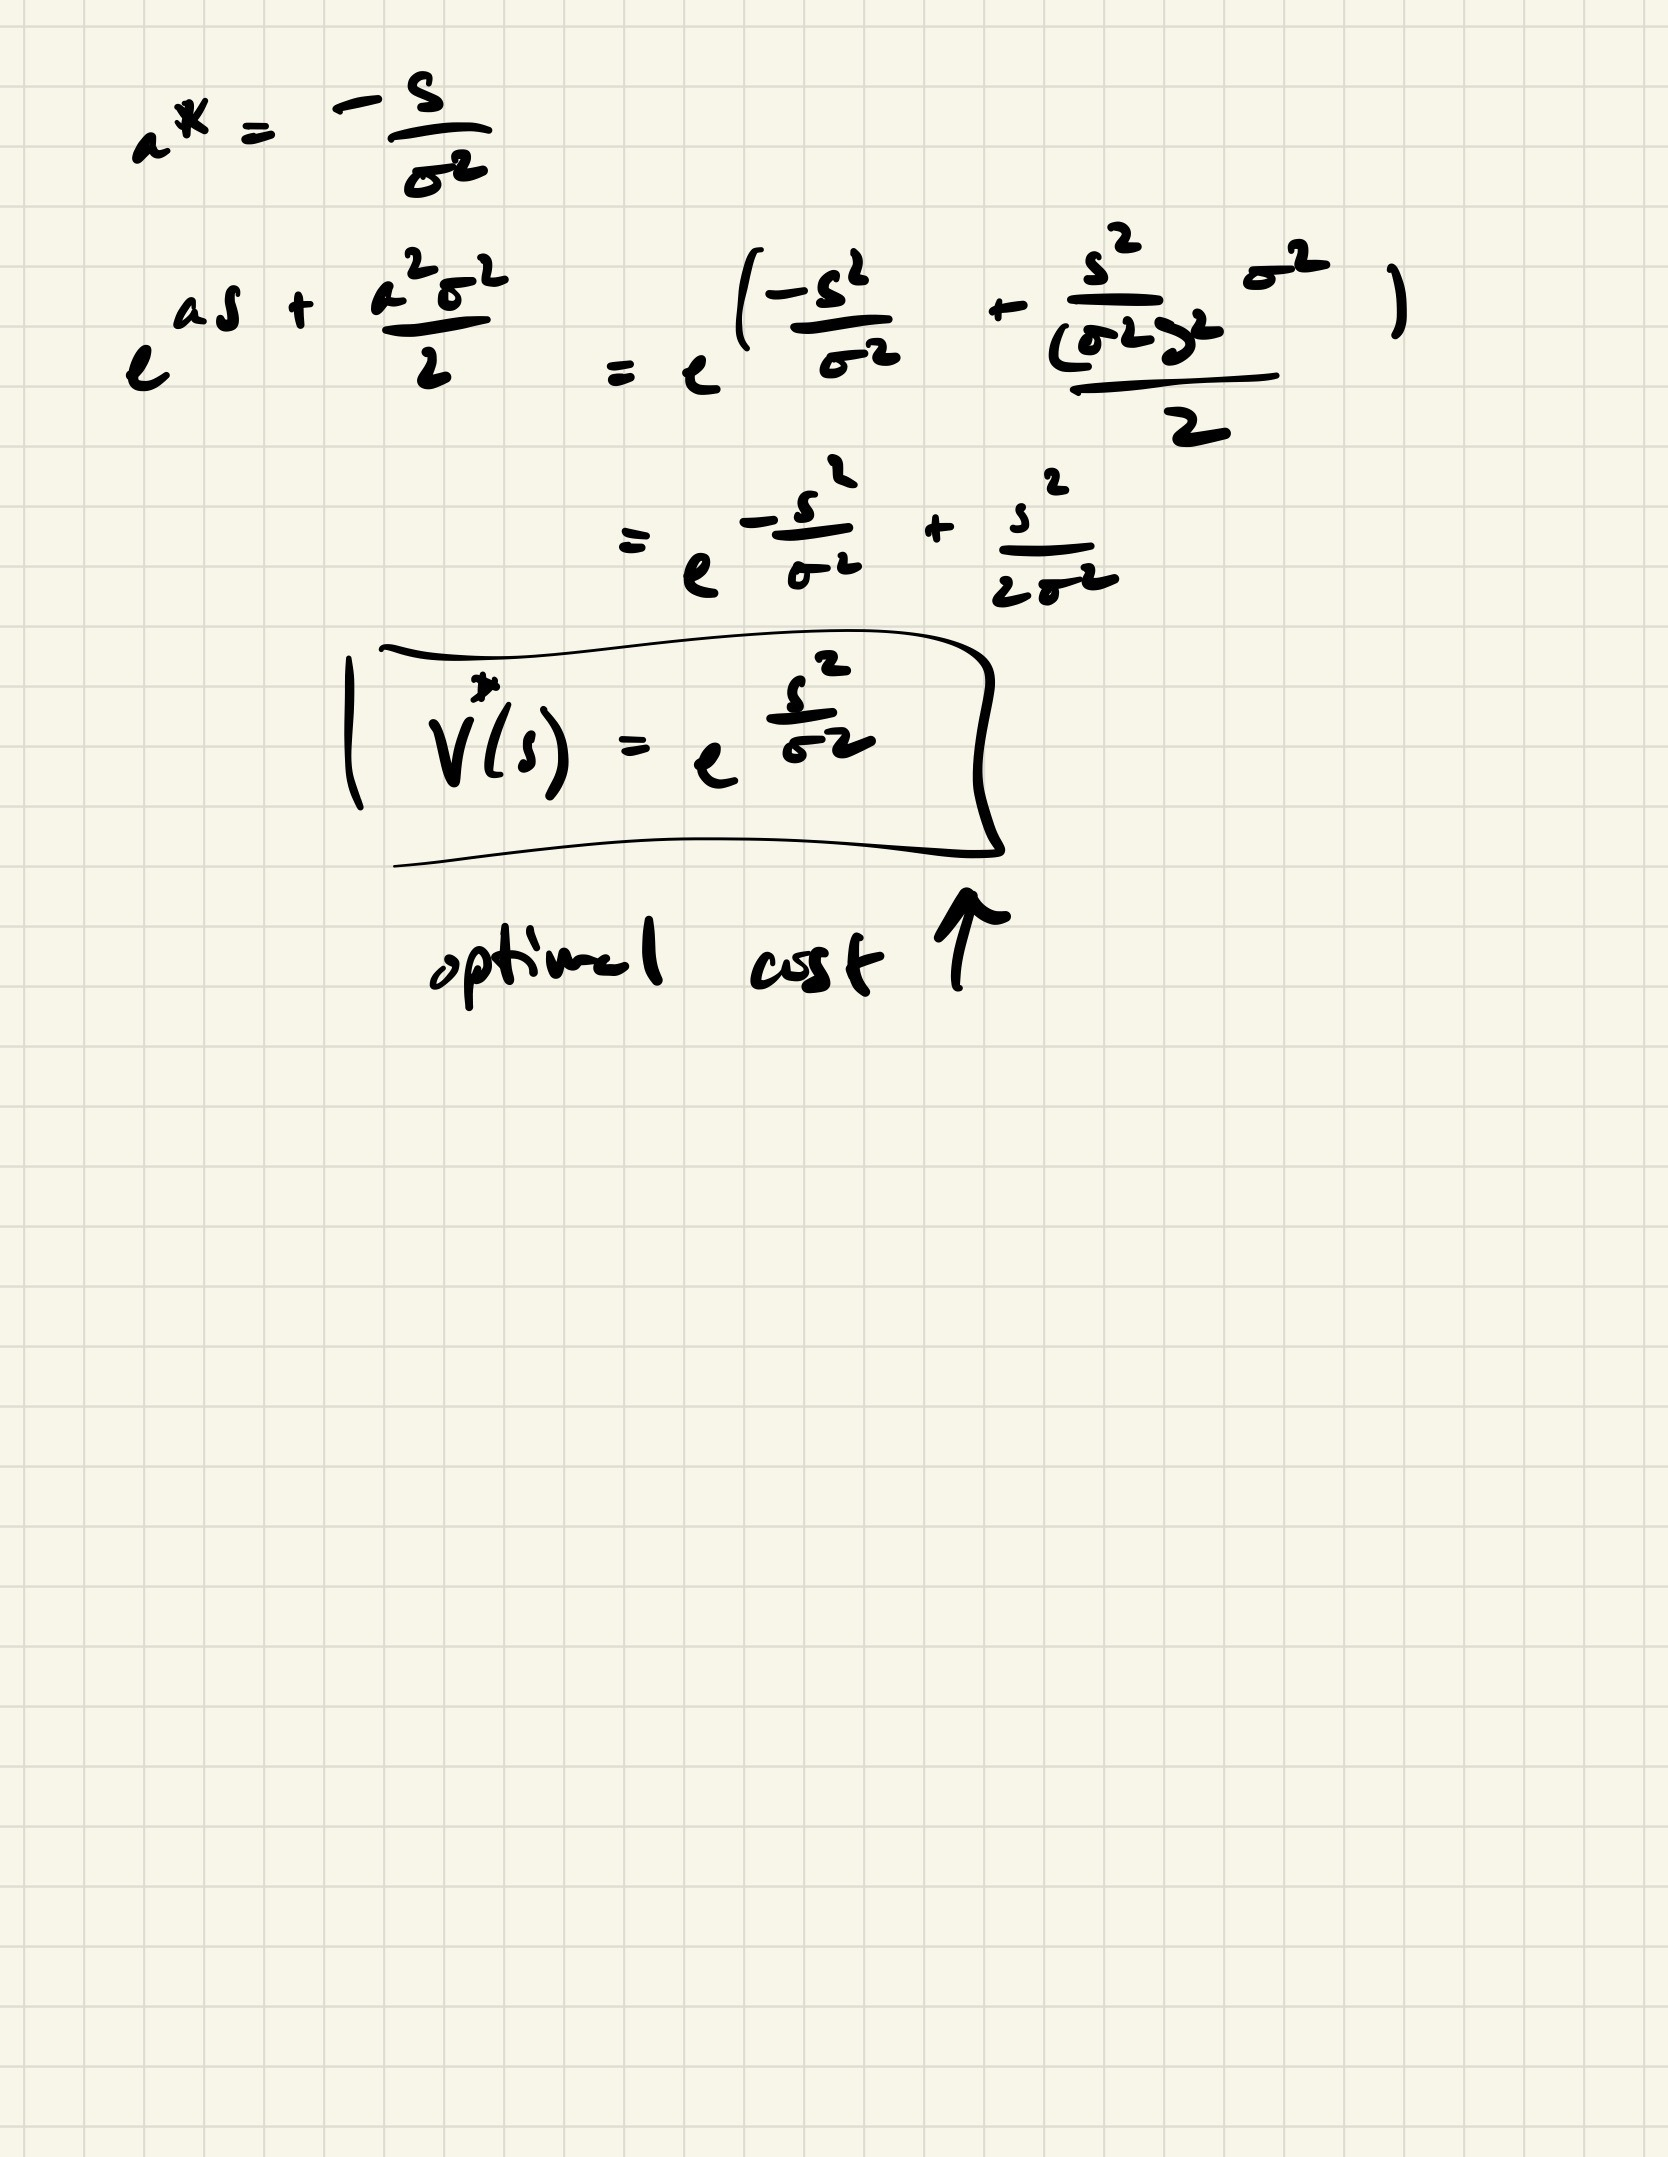
\includegraphics[width=.5\textwidth]{q4_3.jpg}
\end{figure}

\end{document}
